\documentclass[10]{article}
\usepackage[section]{placeins}
\usepackage[T1]{fontenc}
\usepackage[polish]{babel}
\usepackage[utf8]{inputenc}
\usepackage{lmodern}
\selectlanguage{polish}
\usepackage{footmisc}
\usepackage{graphicx}
\usepackage{tikz}
\usepackage{circuitikz}
\usepackage{caption}
\usepackage{afterpage}
\usepackage{subcaption}
\usepackage{enumerate}
\usepackage[margin=0.8in]{geometry}
\usepackage{float}

\renewcommand*{\thefootnote}{\fnsymbol{footnote}}

\def\inputGnumericTable{}  


\begin{document}

\begin{center}
\section*{Ćwiczenie komputerowe z dynamiki molekularnej\\
Monika Seniut\\ 09.11.2016}
\end{center}
\vspace{3cm}
\section{ Wstęp teoretyczny }
Cel ćwiczenia: Nauka tworzenia symulacji dynamiki molekularnej z użyciem algorytmu żabiego skoku, jak również obserwacja przejścia fazowego kryształ - gaz oraz zbadanie własności termodynamicznych charakteryzujących stan gazowy: temperatura, ciśnienie.\\
Przebieg ćwiczenia: Ćwiczenie polegało na zaimplementowaniu symulacji dynamiki molekularnej i wykonaniu eksperymentów/przetestowaniu działania programu dla układu atomów jednego rodzaju oddziaływujących siłami van der Waalsa (model gazu szlachetnego) dla różnych zestawów parametrów wejściowych: 
\begin{itemize}
\item $n$ - liczba atomów wzdłuż każdej krawędzi kryształu ($N ~=~n^3$ - całkowita liczba atomów)
\item $L$ - promień naczynia w kształcie sfery
\item $a$ - odległość między atomami
\item $T_0$ - temperatura początkowa kryształu
\item $\tau$ - krok czasowy
\item $S_o$ - liczba kroków termalizacji
\item $S_d$ - liczba kroków właściwej dynamiki
\item $S_{out}$ - częstotliwość zapisu charakterystyk układu do głównego pliku wyjściowego
\item $S_{xyz}$ - częstotliwość zapisu położeń atomów do pliku XYZ
\end{itemize}
W programie uwzględnione zostało również oddziaływanie atomów ze ściankami naczynia (zachodziło odpychanie atomów od ścianek, dzięki czemu powstawało ciśnienie na atomy argonu).
Dla uproszczenia wszystkie symulacje rozpoczynane były z kryształu romboidalnego o maksymalnym upakowaniu.
W trakcie wykonywania symulacji rejestrowano chwilowe wartości temperatury, ciśnienia, hamiltonianiu oraz energii (T, P, H, V) oraz aktualizowane położenia atomów - współrzędne x, y, z.\\
Program wykonano przy użyciu języka programowania \textit{Python} z użyciem biblioteki \textit{NumPy}. W celu wykonania animacji posłużono się językiem programowania \textit{C++} z użyciem biblioteki \textit{OpenGL}.

\vspace{2cm}
\section{Symulacje}

\subsection{Test programu}
Dla parametrów: $n~=~3$, $a~=~0.38~ nm$, $T_0 ~=~1000~ K$, $L~=~1.2~nm$ sprawdzono zachowanie energii przy kroku $ 10^{-6}\leq \tau \leq 10^{-2}$ i całkowitym czasie symulacji 5ps. Wyniki są przedstawione na rysunku \ref{wykres:(H_av)tau)}. \\
Z zależności $\bar{H}(\tau)$ wynika, iż algorytm jest stabilny dla $\tau \approx 0.004 ~ps$ albo mniejszym. Przy czasach $\tau > 0.004~ps$ wartości średniej energii układu są niefizyczne. Do wykonywania kolejnych symulacji wybrano czas: $\tau~=~0.002~ps$.

\begin{figure}[H]
\begin{center}
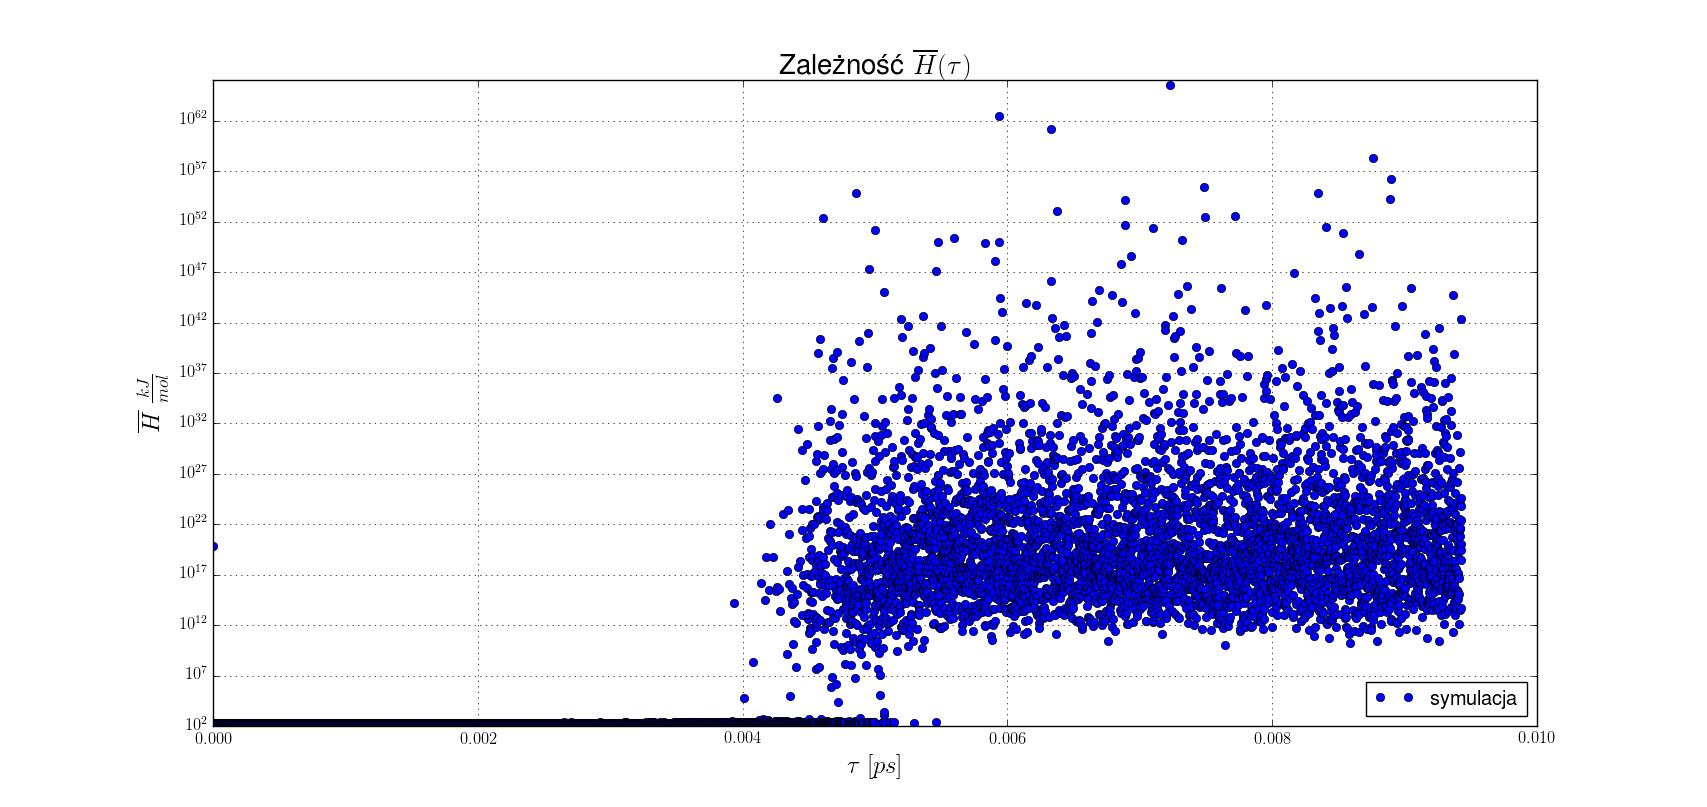
\includegraphics[width=1.\textwidth]{zaleznosc_Hav_od_tau.png}
\caption{Zależnośc średniej energii $\bar{H}$ od kroku $\tau$} \label{wykres:(H_av)tau)}
\end{center}
\end{figure}

\subsection{Krzyształ}
Dla parametrów: $n~=~5$, $a~\approx~0.38~ nm$, $T_0 ~=~0~ K$, $L~=~2.3~nm$ wykonano obliczenia początkowej energii potencjalnej oraz wyznaczono minimum danej energii dla różnych wartości odległości między atomami \textbf{a} w celu znalezienia najlepszego przybliżenia dla danej wartości, przy której początkowa energia potencjalna jest najniższa.

\begin{figure}[H]
\begin{center}
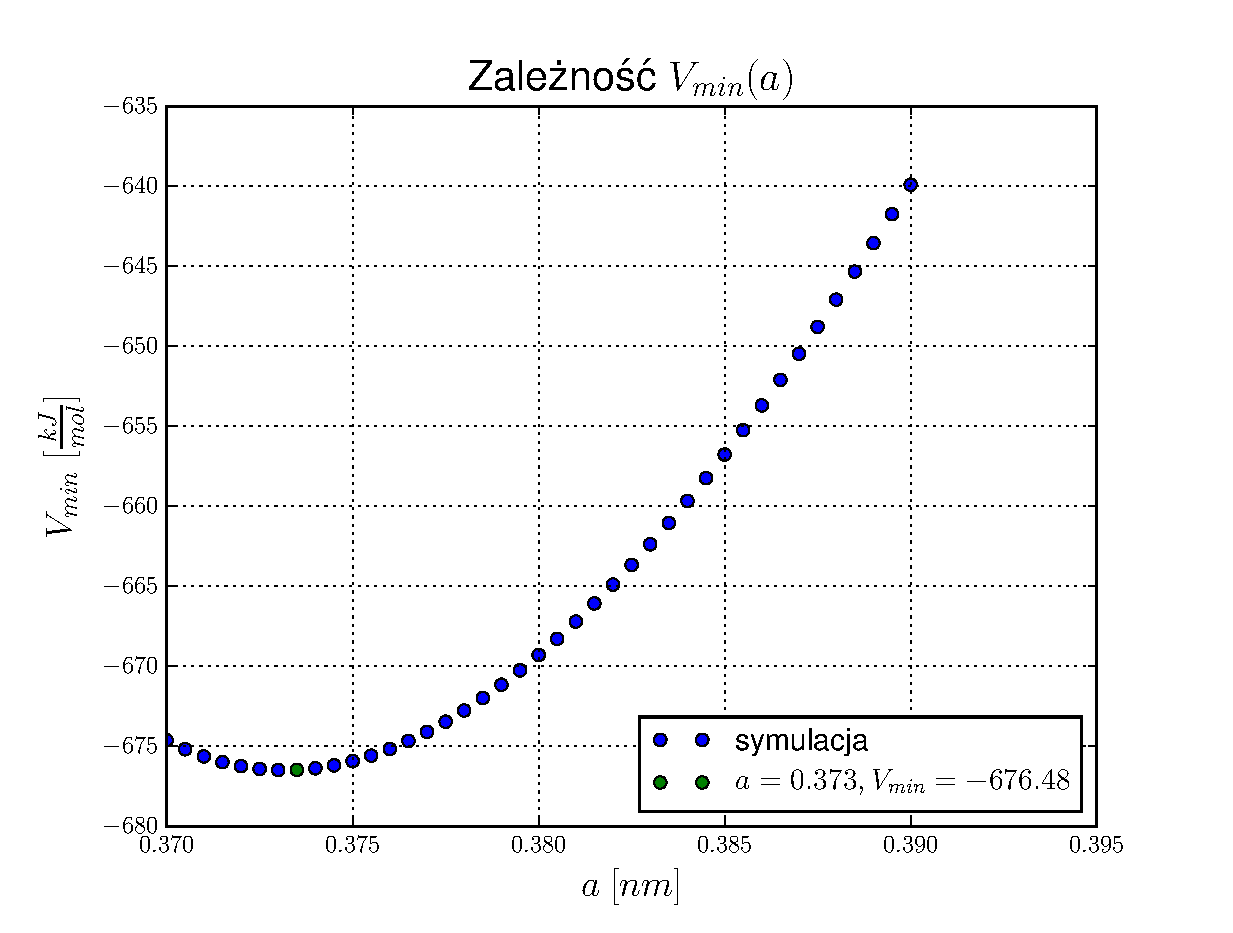
\includegraphics[scale=0.6]{a_minV.eps}
\caption{Zależnośc energii potencjalnej V od odległości międzyatomowej a} \label{wykres:minV(a)}
\end{center}
\end{figure}

Symulację wykonano dla czasu równego \textit{1 ps}. Z wykresu \ref{wykres:minV(a)} widać, iż energia potencjalna przyjmuje minimum dla wartości międzyatomowej \textbf{$a~=~0.373~nm$}, która została ustawiona jako paramter wejściowy do wykonywania kolejnych symulacji w celu uzyskania możliwie najlepszych wyników. Sprawdzono również stabilność kryształu, co przedstawia rysunek \ref{wykres:stabilny}. Średnia temperatura po wykonaniu całej symulacji (czasie 1 ps) wynosiła:\\
\begin{center}
$\bar{T}~\approx~0.1412~ K$
\end{center}
Średnia temperatura kryształu $\bar{T} >~0~K$, ponieważ pomimo tego, iż atomy początkowo są w spoczynku, oddziałują one między sobą siłami van der Waalsa i na skutek tych oddziaływań energia potencjalna jest przekształcana w energię kinetyczną atomów, co można zaobserwować w postaci temperatury, która przyjmuje wartość niezerową.
\begin{figure}[H]
\begin{center}
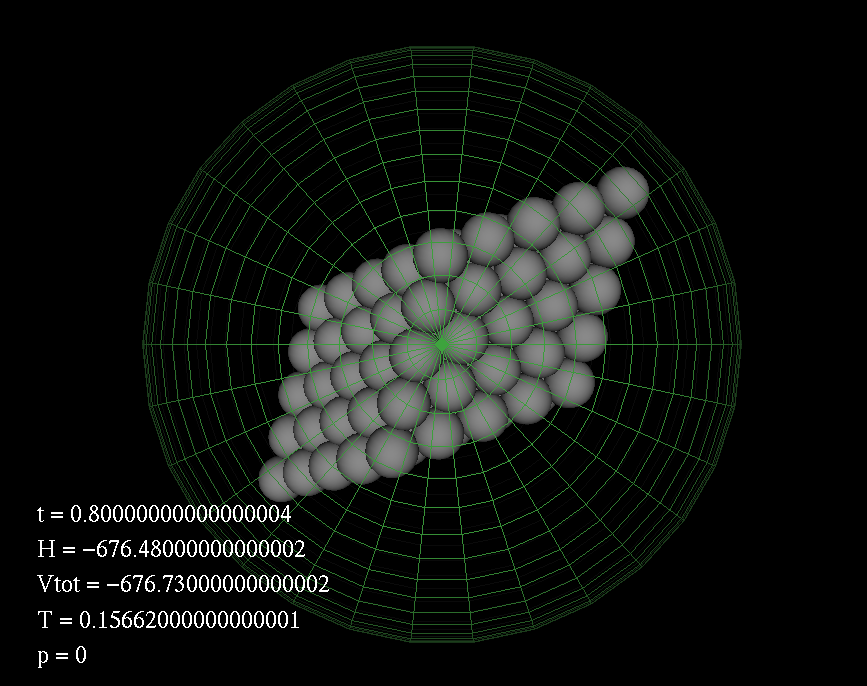
\includegraphics[scale=0.4]{stabilny_T0.png}
\caption{Zdjęcie symulacji dla przypadku $n~=~5$, $a~=~0.373~ nm$, $T_0 ~=~0~ K$, $L~=~2.3~nm$} \label{wykres:stabilny}
\end{center}
\end{figure}

\subsection{Topnienie kryształu}
Dla parametrów: $n~=~5$, $a~=~0.373~ nm$, $L~=~2.3~nm$
%, temperatury początkowej $T_0~=~250~K$ (niższa, żeby mieć możliwość zaobserwowania efektu topnienia kryształu) oraz przy całkowitym czasie symulacji równym textit{6 ps} oszacowano temperaturę topnienia kryształu.
oraz przy różnych ustawieniach początkowej temperatury $T_0$: 200 K, 250 K, 350 K, 400 K oraz całkowitym czasie symulacji \textit{6 ps} na podstawie obserwacji symulacji oszacowano temperaturę topnienia kryształu. Wyniki przedstawiono w tabeli \ref{tabela:oszacowanie T_top}.

\begin{table}[H]
\centering
\begin{tabular}{|l|l|}
\hline
$T_0$ {[}K{]} & $T_{top}$ {[}K{]} \\ \hline
150           &  41        \\ \hline
250          & 57                     \\ \hline
350          &   110            \\ \hline
450          &  210             \\ \hline
\end{tabular}
\caption{Oszacowanie temperatury topnienia kryształu dla różnych temperatur $T_0$}
\label{tabela:oszacowanie T_top}
\end{table}

Jak wynika z tabeli \ref{tabela:oszacowanie T_top} temperatura topnienia kryształu zależy od temperatury początkowej kryształu. Przy temperaturze początkowej $T_0~=~250~K$ temperaturę topnienia z grubsza można oszacować na $55-75 K$.

Metoda szacowania temperatury topnienia kryształu: na podstawie wizualizacji symulacji notowano moment, w którym nie da się już zaobserwować żadnych fragmentów sieci krystalicznej. Taki moment przedstawia rysunek \ref{wykres:topnienie}.

\begin{figure}[H]
\begin{center}
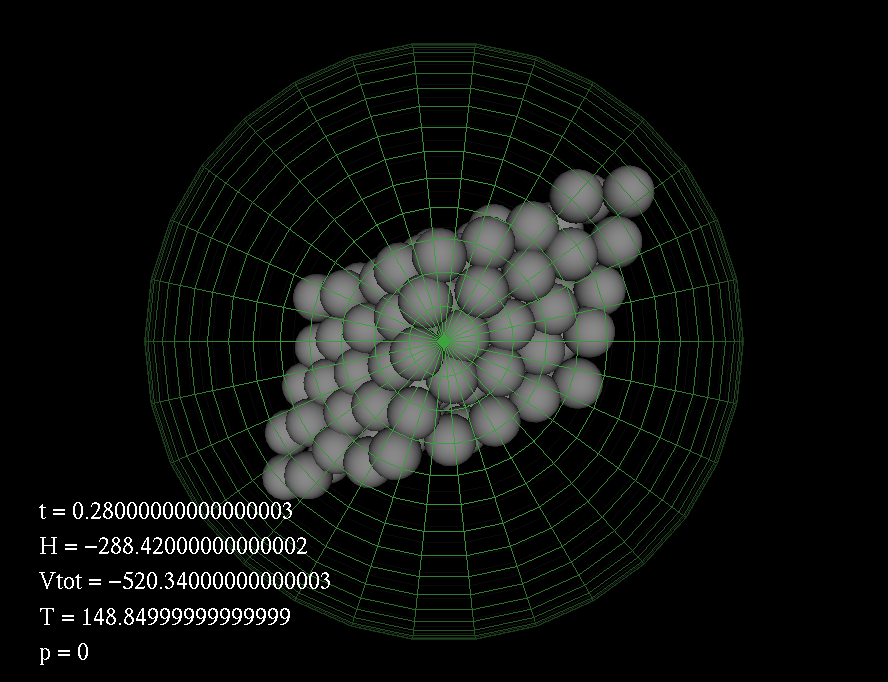
\includegraphics[scale=0.4]{begin.png}
\caption{Początek symulacji dla przypadku $n~=~5$, $a~=~0.373~ nm$, $T_0 ~=~250~ K$, $L~=~2.3~nm$} \label{wykres:begin}
\end{center}
\end{figure}

\begin{figure}[H]
\begin{center}
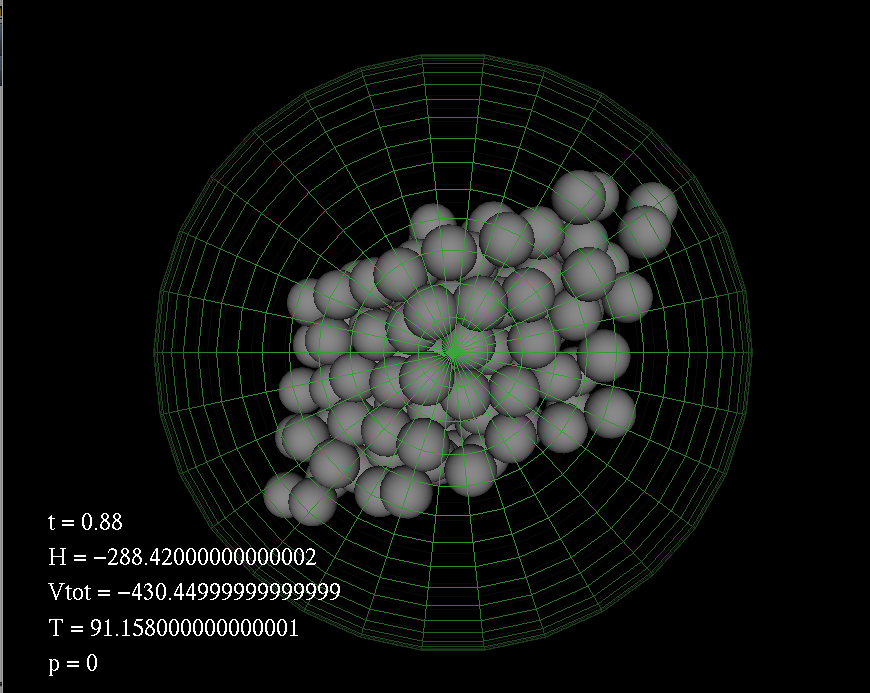
\includegraphics[scale=0.35]{struktura_250.png}
\caption{Moment przed topnieniem kryształu: symulacja dla przypadku $n~=~5$, $a~=~0.373~ nm$, $T_0 ~=~250~ K$, $L~=~2.3~nm$} \label{wykres:poczatek_top}
\end{center}
\end{figure}
Na rysunku \ref{wykres:poczatek_top} jeszcze nie zaszło topnienie kryształu, ponieważ pomimo braku widoczności wyraźnych krawędzi kryształu, widoczne jest jednak kierunkowe ułożenie jego atomów.


\begin{figure}[H]
\begin{center}
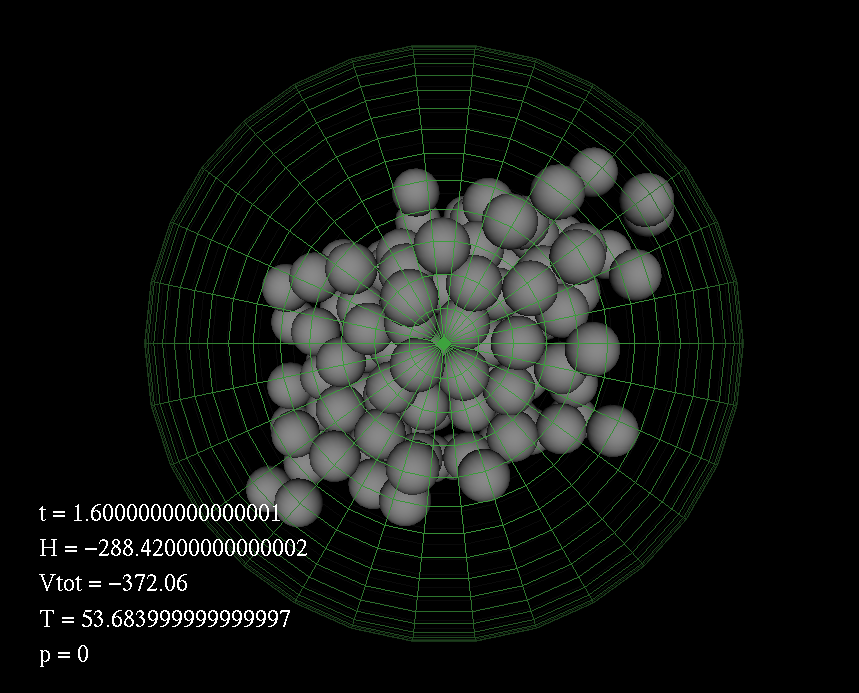
\includegraphics[scale=0.4]{temp_top_250.png}
\caption{Krzyształ po stopieniu: symulacja dla przypadku $n~=~5$, $a~=~0.373~ nm$, $T_0 ~=~250~ K$, $L~=~2.3~nm$} \label{wykres:topnienie}
\end{center}
\end{figure}


\subsection{Gaz}
Dla parametrów: $n~=~5$, $a~=~0.373~ nm$, $L~=~2.3~nm$, $T_0 ~=~1000~ K$ wykonano symulację o całkowitym czasie trwania \textit{6 ps}. Sprawdzono zachowanie temperatury oraz ciśnienia chwilowego, co przedstawiają wykresy \ref{wykres:Tchwil(t)} oraz \ref{wykres:pchwil(t)}. 

\begin{figure}[H]
\begin{center}
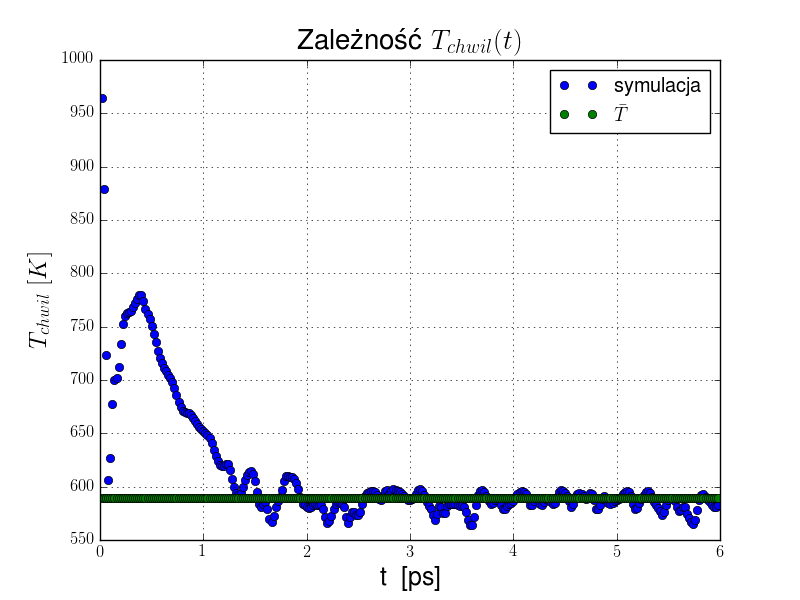
\includegraphics[scale=0.6]{T1000_Tchwil.png}
\caption{Zależność temperatury chwilowej od czasu symulacji dla przypadku $n~=~5$, $a~=~0.373~ nm$, $T_0 ~=~1000~ K$, $L~=~2.3~nm$} \label{wykres:Tchwil(t)}
\end{center}
\end{figure}

\begin{figure}[H]
\begin{center}
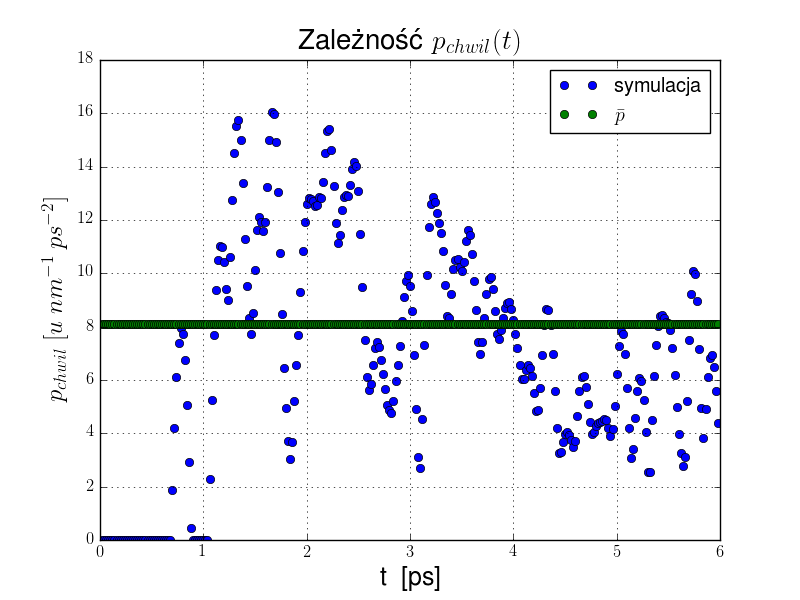
\includegraphics[scale=0.5]{T1000_pchwil.png}
\caption{Zależność ciśnienia chwilowego od czasu symulacji dla przypadku $n~=~5$, $a~=~0.373~ nm$, $T_0 ~=~1000~ K$, $L~=~2.3~nm$} \label{wykres:pchwil(t)}\end{center}
\end{figure}

Z wykresów \ref{wykres:Tchwil(t)} oraz \ref{wykres:pchwil(t)} dla układu o temperaturze początkowej $T_0 ~=~1000~ K$ i całkowitym czasie trwania symulacji \textit{6 ps} wynika, że czas potrzebny na termalizację układu jest nieco większy niż \textbf{1 ps} - wtedy widzimy, że wartości temperatury, jak również ciśnienia stabilizują się i mają tylko nieduże odchylenia wokół swoich wartości średnich.

Dynamikę powtórzono dla 4 wartości $T_0$: 500 K, 1000 K, 1500 K, 2000 K. Na wykresach \ref{wykres:TchwilAll} oraz \ref{wykres:pchwilAll} przedstawionno zależność temperatury chwilowej oraz ciśnienia chwilowego dla danych ustawień temperatury początkowej.

\begin{figure}[H]
\begin{center}
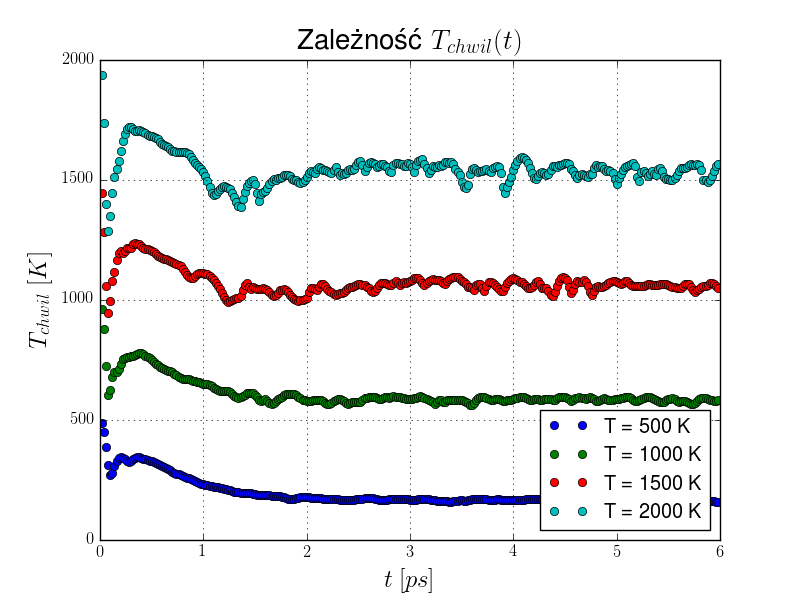
\includegraphics[scale=0.6]{chwiloweT.png}
\caption{Zależność temperatury chwilowej od czasu symulacji dla różnych ustawień $T_0$} \label{wykres:TchwilAll}\end{center}
\end{figure}

\begin{figure}[H]
\begin{center}
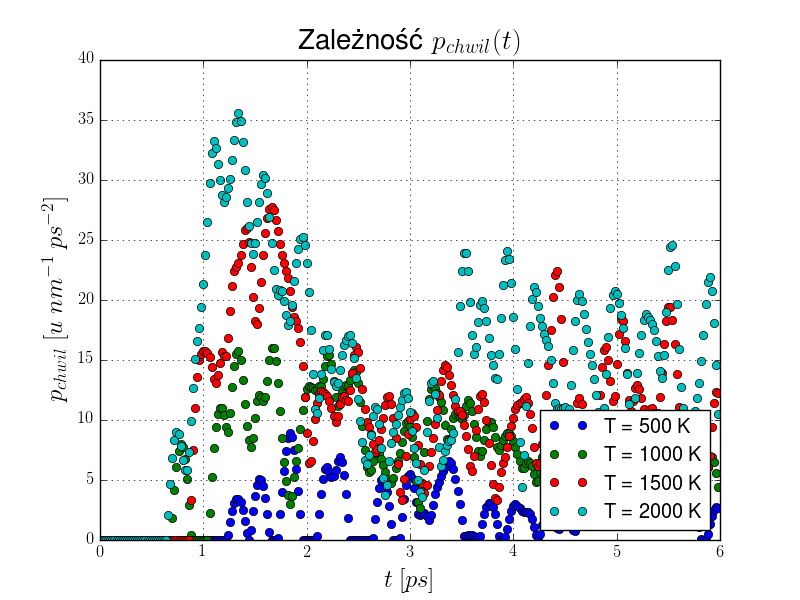
\includegraphics[scale=0.6]{chwiloweP.png}
\caption{Zależność ciśnienia chwilowego od czasu symulacji dla różnych ustawień $T_0$} \label{wykres:pchwilAll}\end{center}
\end{figure}

Z zależności ciśnienia chwilowego lub też zależności temperatury chwilowej od czasu symulacji dla różnych ustawień temperatury początkowej wynika, iż minimalny czas potrzebny na termalizację gazu jest inny - zależny od temperatury początkowej. Im niższa jest dana temperatura, tym więcej czasu układ potrzebuje na termalizację. Np. przy temperaturze $T_0~=~2000~K$ czas ten jest zdecydowanie krótszy niż $1~ps$, natomiast w przypadku $T_0~=~500~K$ czas potrzebny na termalizację jest wyraźnie większy niż $1~ps$.\\
Wniosek: minimalny czas potrzebny na stopnienie kryształu i termalizację gazu jest tym dłuższy im niższa jest temperatura początkowa kryształu.
\\
W celu porównania modelu z gazem doskonałym zbadano zależność średniego ciśnienia gazu od średniej temperatury tego gazu i porównano ją z odpowiednią zależnością dla gazu doskonałego. Porównanie przedstawiono na wykresie zależności $\bar{P}(\bar{T})$: \ref{wykres:clappeyron}.
Wyniki symulacji odbiegają od prostej teoretycznej dla gazu doskonałego tym więcej, im wyższa jest średnia temperatura. Spodziewamy się rozbieżności z powodu skończonych możliwości obliczeń numerycznych oraz założeń modelu. Jednak w danym przypadku rozbieżności są zbyt duże, ale, niestety, przyczyna jest nieznana. 

\begin{figure}[H]
\begin{center}
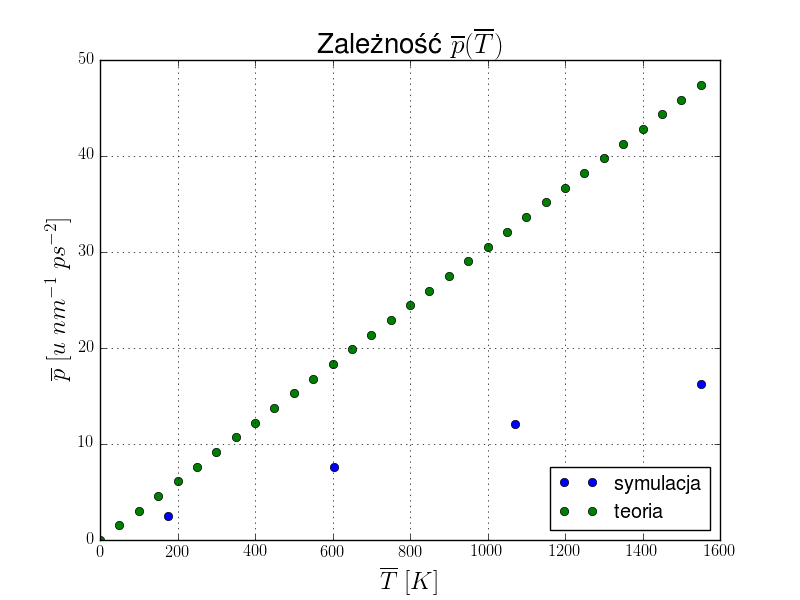
\includegraphics[scale=0.6]{p_av(T_av).png}
\caption{Zależność ciśnienia średniego od średniej temperatury gazu} \label{wykres:clappeyron}
\end{center}
\end{figure}


\end{document}